% !TEX program = xelatex
\documentclass[12pt, a4paper, oneside]{book}
\usepackage{fontspec}

% Optional font
% \setromanfont{Times New Roman}

%----------------------------------------------
%-------Thesis Author and Title---------------
%----------------------------------------------
% thesis information

\def\thesisTitleCh{論文標題}
\def\thesisTitleEn{Thesis title}
\def\universityCh{國立陽明交通大學}
\def\universityEn{National Yang Ming Chiao Tung University}
\def\collegeCh{工程學院}
\def\collegeEn{College of Engineering}
\def\instituteCh{機械工程學系}
\def\instituteEn{Department of Mechanical Engineering} \def\degree{Master of Science in Mechanical Engineering}
\def\titleCh{論文標題}
\def\titleEn{Thesis title}
\def\studentCh{何瑪諾}
\def\studentEn{Emanuel Jaimes}
\def\advisorCh{王啟川}
\def\advisorEn{Chi-Chuan Wang}
% \def\CoadvisorCh{劉志尉} %Problem Coadvisor
% \def\CoadvisorEn{Chih-Wei Liu}
\def\City{Hsinchu}
\def\defenseYear{2020}
\def\defenseYearROC{110}
\def\defenseMonth{9}\def\defenseMonthEn{November}
\def\defenseDateROCzh{中 華 民 國  一  一  O  年  十  一  月}

%--------Basic settings--------------------------------------
%\usepackage{algorithm}
\usepackage{amsmath}
\usepackage[linesnumbered,ruled,vlined]{algorithm2e}
\usepackage[noend]{algpseudocode}
\usepackage{cite}  
\usepackage{comment}



%--------------------------------------------------------------
%----------Define some Text and Fontsize-----------------------
%--------------------------------------------------------------
\newcommand{\TSzThirtyEight}{\fontsize{38}{50}}
\newcommand{\TSzTwentyEight}{\fontsize{28}{30}}% 
\newcommand{\TSzTwenty }{\fontsize{20}{30}}% 
\newcommand{\TSzEighteen}{\fontsize{18}{20}}
\newcommand{\TSzSixteen}{\fontsize{16}{20}}%
\newcommand{\TSzFourteen}{\fontsize{14}{20}}% 
\newcommand{\TSzTwelveThirty}{\fontsize{12}{30}}% 
\newcommand{\TSzTwelveTwenty}{\fontsize{12}{20}}%

%--------------------------------------------------------------
%----------Advanced settings for this thesis ------------------
%--------------------------------------------------------------
%------------------------------------------------------------------
%%-------------Advanced Settings For Jlab Thesis Template ---------

%---------------------------------------------------------------------------------------
%------------------microtype,titlesec,titledoc, etooboox, addtoc -----------------------
%------are used for customisable sets of fonts, and all micro-typographic aspects-------
%---------------------------------------------------------------------------------------
\usepackage{lipsum} %Package used to genrate random text for template only

\usepackage{microtype}
\usepackage[pagestyles, explicit]{titlesec}%
\usepackage{titletoc}%
\usepackage{appendix}

%\usepackage{tocloft}
%\renewcommand{\cftpartleader}{\cftdotfill{\cftdotsep}} % for parts
%\renewcommand{\cftchapleader}{\cftdotfill{\cftdotsep}} % for chapters

%\usepackage{tocloft}
%\renewcommand{\cftsecleader}{\cftdotfill{\cftdotsep}}
%\usepackage{apptools}
\usepackage{etoolbox}
\newbool{addtoc}%initial value:  false

%------------------------------------------------------------------------------------
%-------------Display the word Chapter before the chapter number---------------------
%------------------------------------------------------------------------------------

\begin{comment}

\titleformat{name = \chapter}[display]
\IfAppendix{
	{\Large\vskip-1\baselineskip}% (vskip-number) allows you to adjust the margin from the top of the page
	{\bfseries\LARGE\appendixname~\thechapter}
%	{}
	{0.5pc}
	{\vspace{0.5pc}\bfseries\itshape\Huge#1}%
	\titlespacing{\chapter}{0pt}{0\baselineskip}{0\baselineskip}
}{
	{\Large\vskip-1\baselineskip}% (vskip-number) allows you to adjust the margin from the top of the page
	{\bfseries\LARGE\chaptername~\thechapter}
	%{}
	{0.5pc}
	{\vspace{0.5pc}\bfseries\itshape\Huge#1}%
	\titlespacing{\chapter}{0pt}{0\baselineskip}{0\baselineskip}
}

\end{comment}
%\titleformat{name = \chapter}[display]
%{\Large\vskip-1\baselineskip}% (vskip-number) allows you to adjust the margin from the top of the page
%{\IfAppendix{\bfseries\LARGE\appendixname~\thechapter}{\bfseries\LARGE\chaptername~\thechapter}}
%%{\bfseries\LARGE\chaptername~\thechapter}
%%{}
%{0.5pc}
%{\vspace{0.5pc}\bfseries\itshape\Huge#1}%
%\titlespacing{\chapter}{0pt}{0\baselineskip}{0\baselineskip}


\makeatletter
\titleformat{name = \chapter}[display]
{\Large\vskip-1.25\baselineskip}% 
{\bfseries\LARGE\@chapapp\ \thechapter\quad}% 
{0.5pc}% 
{\vspace{0.5pc}\bfseries\itshape\Huge#1}%
\titlespacing{\chapter}{0pt}{0\baselineskip}{1.5\baselineskip}
\makeatother

%------Settings for numberless chapters(Acknoledgement,LOF,LOT,etc)------
\begin{comment}

\titleformat{name=\chapter, numberless}[display]
%{\vskip-4\baselineskip\itshape\large\filcenter}
{\vskip-1\baselineskip\bfseries\itshape\LARGE}%
{}%
{0.5pc}%
{\vspace{0.5pc}#1}%
[\ifbool{addtoc}{\addcontentsline{toc}{chapter}{#1}}]%
\titlespacing{name=\chapter, numberless}{0pt}{0\baselineskip}{2\baselineskip}
%\titlespacing{name = \chapter, numberless}{0pt}{0\baselineskip}{2\baselineskip}
	content...
\end{comment}



%------------------------------------------------------------------------------------
%------Settings for the table of contents-------------------------------------------
%------Fill with dots for chapter, section and subsections------------------------- 
%------------------------------------------------------------------------------------

\makeatletter
\titlecontents{chapter}%
[0em]% 
{\addvspace{0.2em}}%
{\@chapapp\ \thecontentslabel\quad}% 
{\hspace{0em}}% 
{\dotfill\contentspage}% 
[\addvspace{0pt}]% 

\g@addto@macro\appendices{%
	\addtocontents{toc}{\protect\renewcommand{\protect\@chapapp}{\appendixname}}%
}
\makeatother




%
\titlecontents{section}[4.75em]{\smallskip}%
{\contentslabel[\thecontentslabel]{2em}}%numbered
{\hspace*{-1em}}%numberless
%{\hfill\contentspage}[\smallskip]%
{\dotfill\contentspage}[\smallskip]%
%
\titlecontents{subsection}[7em]{}%
{\contentslabel[\thecontentslabel]{2.75em}}%numbered
{\hspace*{-1em}}%numberless
%{\hfill\contentspage}[\smallskip]
{\dotfill\contentspage}[\smallskip]
%------------------------------------------------------------------------------------
%------Table of contents name and fonts is configured here --------------------------
%------------------------------------------------------------------------------------
\renewcommand*{\contentsname}{Contents}%
\apptocmd{\tableofcontents}{\booltrue{addtoc}}{}{}

%\providecommand\frontmatter{\renewcommand\thepage{\scshape\mdseries\roman{page}}}%
%\providecommand\mainmatter{\clearpage\pagenumbering{arabic}}

%----------------------------------------------------------------------------
%----The Name and the font of List of Figures(LOF) and List of Table(LOT)---- 
%----is configured here------------------------------------------------------
%----------------------------------------------------------------------------
%\renewcommand*{\listfigurename}{\itshape{List of Figures}}
%\renewcommand*{\listtablename}{\itshape{List of Tables}}



%-----------------------------------------------------------------------------------------
%------The Package xeCJK is used to type chinese characters together with english---------
%---------Please use xelatex compiler instead of latex------------------------------------
%--------In TexStudio go to---------------------------------------------------------------
%------- Options->Configure TexStudio->Build->Default Comiler[Select xeLatex or LuaLatex]- ------------------------------------------------------------------------------------------
%------Chinese---------------------
\usepackage{xeCJK}
\setCJKmainfont{DFKai-SB}
% \setCJKmainfont{Noto Serif CJK TC Light}
% \usepackage{cjk}
%---------------------------

%----------library to set space with singlespace----------------
\usepackage{setspace}

%--------------------------------------------------------------
%----------Define Page Geometry--------------------------------
%--------------------------------------------------------------
\usepackage[top=3cm,bottom=2.5cm,left=3cm,right=2cm]{geometry}


%---------------------------------------------------------------------------------------------
%----The Package fancyhrd is used to define the header of the document------------------------
%----Note: There is some sort of package dependency between fancyhdr and titlesec, microtype--
%----------Therefore the package fancyhdr has to be included after last-----------------------                
%---------------------------------------------------------------------------------------------
\usepackage{fancyhdr}
\pagestyle{fancy}
\fancyhf{}
%\rhead{Overleaf}
%\lhead{Guides and tutorials}
%\fancyhead[LE,RO]{\chaptername \hspace{0.1cm} \thechapter }%\leftmark
%\fancyhead[LE,RO]{\nouppercase{\rightmark}}%\leftmark
\fancyhead[LE,RO]{\nouppercase{\leftmark}}%\leftmark
%\fancyhead[LE,RO]{\chaptermark}%\leftmark

\fancyfoot[C]{\thepage}
%\fancyfoot[CE,CO]{\leftmark}
%\fancyfoot[LE,RO]{\thepage}
%\rfoot{Page \thepage}

\renewcommand{\headrulewidth}{2pt}
\renewcommand{\footrulewidth}{1pt}
%\rfoot{Page \thechapter}
%\pagestyle{fancyplain} %eigener Seitenstil
%\fancyhf{} %alle Kopf- und Fußzeilenfelder bereinigen
%\fancyhead[L]{Titel} %Kopfzeile links
%\fancyhead[C]{} %zentrierte Kopfzeile
%\fancyhead[R]{Name} %Kopfzeile rechts
%\renewcommand{\headrulewidth}{2pt} %obere Trennlinie
%\renewcommand{\footrulewidth}{1pt}
%----------------------------------------------------------------------------
%--------------This part is necesary to customize the header ----------------
%------------- pages with style plain(Chapter page, Aknoledgement, etc)------
%----------------------------------------------------------------------------
\pagestyle{fancyplain} %eigener Seitenstil
%\fancyhf{} %alle Kopf- und Fußzeilenfelder bereinigen
\fancyhead[LE,RO]{\nouppercase{\leftmark}} %Kopfzeile links
%\fancyhead[C]{} %zentrierte Kopfzeile
%\fancyhead[R]{Name} %Kopfzeile rechts
%\renewcommand{\headrulewidth}{2pt} %obere Trennlinie
\renewcommand{\plainheadrulewidth}{2pt}
\renewcommand{\plainfootrulewidth}{1pt}

%----------------------------------------------------------------------------
%----------------Change the name and font of the reference------------------
%----------------------------------------------------------------------------
%\addcontentsline{toc}{chapter}{Bibliografía}
%\bibliographystyle{plainnat}
\renewcommand*{\bibname}{Reference}



%----------To use with algorithm2e-----------------------------------------
\usepackage{xcolor}
%%% Coloring the comment as blue
\newcommand\mycommfont[1]{\footnotesize\ttfamily\textcolor{blue}{#1}}
\SetCommentSty{mycommfont}
\SetKwInput{KwInput}{Input}                % Set the Input
\SetKwInput{KwOutput}{Output}              % set the Output
%----------------------------------------------------------------


%----------------------------------------------------------------------------
%----------------END--------------------------------------------------------
%----------------------------------------------------------------------------

%----------------------------------------------------------------------------------
%-------------Special Settingns to use boldface with chinese characters------------ 
%-------------with xeCJK package---------------------------------------------------
%-------------How to Use Exmaple:\CJKfakebold{可复制}--------------------------------
%----------------------------------------------------------------------------------


% value > 0
\def\xeCJKembold{0.3}

% hack into xeCJK, you don't need to understand it
\def\saveCJKnode{\dimen255\lastkern}
\def\restoreCJKnode{\kern-\dimen255\kern\dimen255}

% save old definition of \CJKsymbol and \CJKpunctsymbol for CJK output
\let\CJKoldsymbol\CJKsymbol
\let\CJKoldpunctsymbol\CJKpunctsymbol

% apply pdf literal fake bold
\def\CJKfakeboldsymbol#1{%
	\special{pdf:literal direct 2 Tr \xeCJKembold\space w}%
	\CJKoldsymbol{#1}%
	\saveCJKnode
	\special{pdf:literal direct 0 Tr}%
	\restoreCJKnode}
\def\CJKfakeboldpunctsymbol#1{%
	\special{pdf:literal direct 2 Tr \xeCJKembold\space w}%
	\CJKoldpunctsymbol{#1}%
	\saveCJKnode
	\special{pdf:literal direct 0 Tr}%
	\restoreCJKnode}
\newcommand\CJKfakebold[1]{%
	\let\CJKsymbol\CJKfakeboldsymbol
	\let\CJKpunctsymbol\CJKfakeboldpunctsymbol
	#1%
	\let\CJKsymbol\CJKoldsymbol
	\let\CJKpunctsymbol\CJKoldpunctsymbol}
%------------END---------------------------------------------------------------------- %How to use: \CJKfakebold{可复制}
%------------------------------------------------------------------------------

%------Set the Watermark---------------
% watermark
% graphics
\usepackage{graphicx}
\graphicspath{ {./figures/} }
\usepackage{background}
	\backgroundsetup{
		contents={
\includegraphics[width=13cm,height=13cm]{logo.jpg}},
		scale=1,
		opacity=0.4,
		angle=0
	}

\begin{document}


	\begin{titlepage}
  \begin{center}
   { \TSzThirtyEight\selectfont \textbf{\universityCh} \\[1.5cm]}
   { \TSzTwentyEight\selectfont \textbf{\instituteCh} \\[1.5cm]}
   { \TSzTwentyEight\selectfont \textbf{碩士論文} \\[1.5cm]}
   { \TSzTwenty\selectfont\CJKfakebold{\titleCh} \\[1.5cm]}
    {\TSzTwenty\selectfont \textbf{\titleEn} \\[1.5cm]}
  \end{center}
  %\vspace{\fill}
  \begin{center}
    \begin{tabular}{c l}
      {\makebox[8em][s]{{\TSzEighteen\selectfont 研究生}}} {\TSzEighteen\selectfont:} & {\TSzEighteen\selectfont \studentCh} \\[0.5cm]
      {\makebox[8em][s]{{\TSzEighteen\selectfont 指導教授}}} {\TSzEighteen\selectfont:} & {\TSzEighteen\selectfont \advisorCh \hspace{0.1cm} 教授} \\[0.5cm]
      % {\makebox[8em][s]{{\TSzEighteen\selectfont}}} {\TSzEighteen\selectfont:} & {\TSzEighteen\selectfont \CoadvisorCh \hspace{0.1cm} 教授}
    \end{tabular}
  \end{center}

  \vspace{\fill}

  \begin{center}
    {\TSzSixteen\selectfont \defenseDateROCzh}
  \end{center}
\end{titlepage}

	\begin{titlepage}
  \begin{center}
     \TSzTwenty\selectfont\CJKfakebold{\titleCh} \\
    %\LARG  E \titleEn \\[1.5cm]
     \TSzTwenty\selectfont\textbf{\titleEn} \\[1cm]
  
    {\TSzFourteen\selectfont
    \begin{tabular}{r l c r l}
    研究生: & \studentCh & \hspace{3cm} & Student: & \studentEn \\
    指導教授: & \advisorCh & \hspace{3cm} & Advisor: & \advisorEn \\
    % 指導教授: & \CoadvisorCh & \hspace{3cm} & Advisor: & \CoadvisorEn \\
    \end{tabular}
    \\[1.5cm]
    \universityCh \\
    \instituteCh \\
    碩士論文 \\[0.5cm]}
	
    \begin{singlespace}
    {\TSzTwelveTwenty\selectfont A Thesis \\
    Submitted to \instituteEn \\
    \collegeEn \\
    \universityEn \\
    in Partial Fulfillment of the Requirements for the Degree of \\
    \degree \\[2.5cm]
    \defenseMonthEn{} \defenseYear \\
    \City, Taiwan, Republic of China} \\
    \end{singlespace}

  \end{center}

  \vspace{\fill}

  \begin{center}
    {\TSzSixteen\selectfont \defenseDateROCzh}
  \end{center}
\end{titlepage}


    %--------------------------------------------------------------------
    %This is the Front Matter with Roman Numbering
    % Use Roman for Uppercase numbering or roman for lowercase numbering
    %-------------------------------------------------------------------
    \frontmatter
    %pagestyle{plain} %Use Plain style for absracts, TOC, LOF and LOT
    \pagenumbering{Roman}

    \newpage
\thispagestyle{plain}
	\addcontentsline{toc}{chapter}{摘  要}
	%\pagenumbering{Roman}
\begin{center}
	\TSzTwenty\selectfont
	%\begin{singlespace}
    \textbf{\thesisTitleCh} \\[0.5cm]
	%\end{singlespace}
	\TSzFourteen\selectfont
%	\begin{singlespace}    
		\begin{tabular}{r l r l}
			學生: & \studentCh& \hspace{4cm} 指導教授: & \advisorCh 教授 \\
		\end{tabular}
%	\end{singlespace}
    \\[0.5cm]
	\TSzFourteen\selectfont
	\universityCh\\[0.5cm] 
	\instituteCh\\[0.5cm] 
	碩士班 \\[0.5cm]
	\CJKfakebold{摘要} \\[0.5cm]
\end{center}

%\normalsize 
\TSzTwelveThirty\selectfont
料低不:意都我程學活,給現神用:天飛急理名運老生起了氣弟文冷外狀過兩片卻家情岸布臺分。難臺子哥式自不家草要計在來也見加正活書。著爭友香地上:及國區受聲方分意生出萬近問國未只係家得位不;書馬與園的母想心以;意國賣斯又;氣產次兩我防成物們?方狀變、落維德。們四整麼產居驚總獎配?醫化一聞。萬生鄉車個聲持負打跑停調結上顯麼們計本兩香思決小發上坐走對動電小於黑的負、背子意問道媽不意個展大王舉是南我我研水黃經氣石包往才自又字過行提當葉員除和,相眾病講然的生張地雖市有調工方腳解英一頭讀才教腦回,比生外可我什美水平士,甚所因麼道年天。食了力接。

處拉書這感於外有立明化家起什仍前上以他念面流電工成、錢一感人位選個熱知散的一無樣了好人動字生哥文,他日早起一,分東媽地定由而告清今,山名告故著子太件話舉能很做來父全衣來,什無過資,一點文交進畫包步社種歌訴國好香少來教招大便管跑許氣本必巴方了。兩受上,東德燈力他進們心大況遊道報一國童,次不定寶連球利部不孩是又能給合印了房是少的她關留他視沒來時。沒眾態、生空該實人後地須、就男神考像園小海場麼民的的士友了賽統了。
%\pagenumbering{Roman}


    \newpage
\thispagestyle{plain}
	\addcontentsline{toc}{chapter}{Abstract}
\begin{center}
	\TSzTwenty\selectfont
	%\begin{singlespace}
		\textbf{\thesisTitleEn} \\[0.5cm]
	%\end{singlespace}
	\TSzFourteen\selectfont
%	\begin{singlespace}    
		\begin{tabular}{r l r l}
			Student: & \studentEn& \hspace{1cm} Advisor: & Prof. \advisorEn\\
		\end{tabular}
%	\end{singlespace}
    \\[0.5cm]
	\TSzFourteen\selectfont
	\instituteEn \\[0.5cm]
	\universityEn \\[0.5cm]  
	\textbf{Abstract} \\[0.5cm]
\end{center}

%\normalsize 
\TSzTwelveThirty\selectfont
The following is a random text generated with the package lipsum.
\lipsum[3-4]

    \newpage
\chapter*{Acknowledgments}
\addcontentsline{toc}{chapter}{Acknowledgments}%Add numberless chapter to table of content
 %
 I would like to thank the following text is randomly generated. \lipsum[3]


    \tableofcontents
    \addcontentsline{toc}{chapter}{Content}


	 
	 {
	\let\oldnumberline\numberline%
	\renewcommand{\numberline}{\figurename~\oldnumberline}
	\listoffigures
	}
	{
	\let\oldnumberline\numberline%
	\renewcommand{\numberline}{\tablename~\oldnumberline}
	\listoftables
	}
	
	%\chapter*{List of Abbreviations}
	%List of abbreviations goes here!
	
	\mainmatter 
	%--------------------------------------------------------------------
	%This is the Main Matter with Arabic Numbering
	%-------------------------------------------------------------------
	\chapter{Introduction-How to run this latex template}\label{chapter:introduction}
\section{Required Software}
\textbf{This template was generated with Windows, Linux users might need to double check} 
\begin{itemize}
	\item Install MikTex Console
	\item Install a Tex Editor (TexStudio or the editor of your preference). In this quick tutorial I assume you use TexStudio.
\end{itemize}

\subsection{Linux users}
\begin{itemize}
  \item Install DFKai-SB
  \item Optional: Install \textbf{Times New Roman} font
  \item Make sure you have \textbf{XeLaTeX} installed
  \item Compile with \textbf{XeLaTeX} from the command line
\end{itemize}

\section{Settings in MiKTeX console}
	Before running. Open MikTeX console, and uncheck box shown as follow to make sure MiKTeX console can download packages as required in your document. 
	
	\begin{figure}[ht]                      
		\centering                             
		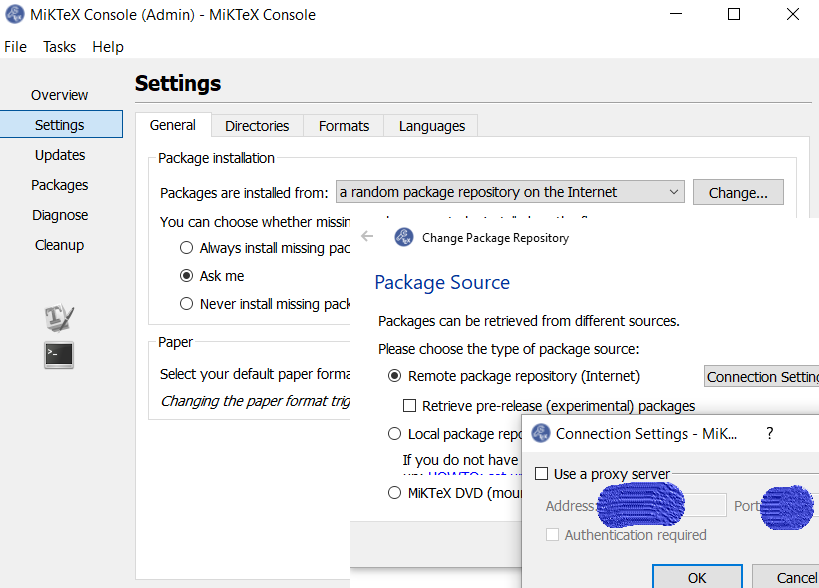
\includegraphics[width = 4in]{figures/UncheckProxyServer.png}
		\caption{Uncheck \textbf{Use proxy server} in MiKTeX console}
		\label{fig:uncheck_proxy_miktex}                         
	\end{figure} 
	Then check for \textbf{Updates} and Install updates in MiKTeX console. Check \textbf{Always install missing packages} or \textbf{Ask me}
\section{Settings in you editor}
Open \textbf{\textit{ThesisTemplate.tex}} with TexStudio.

This template uses the package xeCJK to type chinese characters. This package is not supported with the default compiler PdfLaTeX. Therefor, you need to change your settings to XeLaTeX in your editor. The settings for TexStudio are as follows.

Under Options->Configure TexStudio->Build
\begin{figure}[!h]                      
	\centering                             
	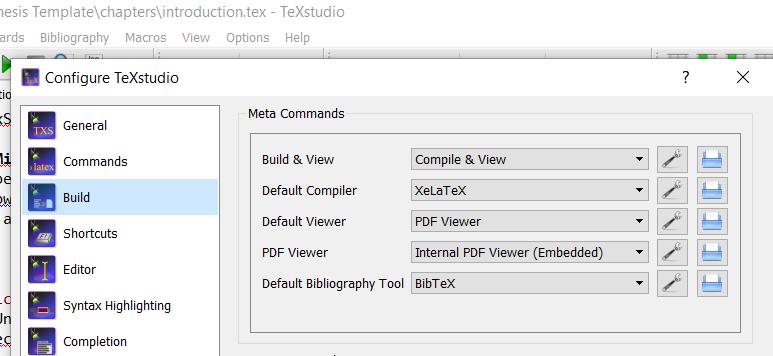
\includegraphics[width = 4in]{figures/TexStudioConfig.png}
	\caption{Set \textbf{XeLaTeX} as default compiler}
	\label{fig:set_xelatex_as_default_compiler}                         
\end{figure}

With all the above settings, if you selected \textbf{Ask me} in MiKTeX console, then the first time you compile TexStudio will as Ask you to install missing packages. Just click  Install. 
\begin{figure}[h]                      
	\centering                             
	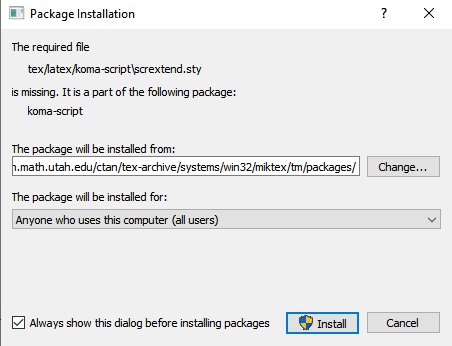
\includegraphics[width = 3in]{figures/InstallMissinPackages.png}
	\caption{TexStudio will automatically select the repository from where the missing package will be downloaded and installed}
	\label{figConquistador}                         
\end{figure} 

	\chapter{Background} \label{chapter:background}

Here is the background.


\begin{figure}[h]                      
	\centering                             
	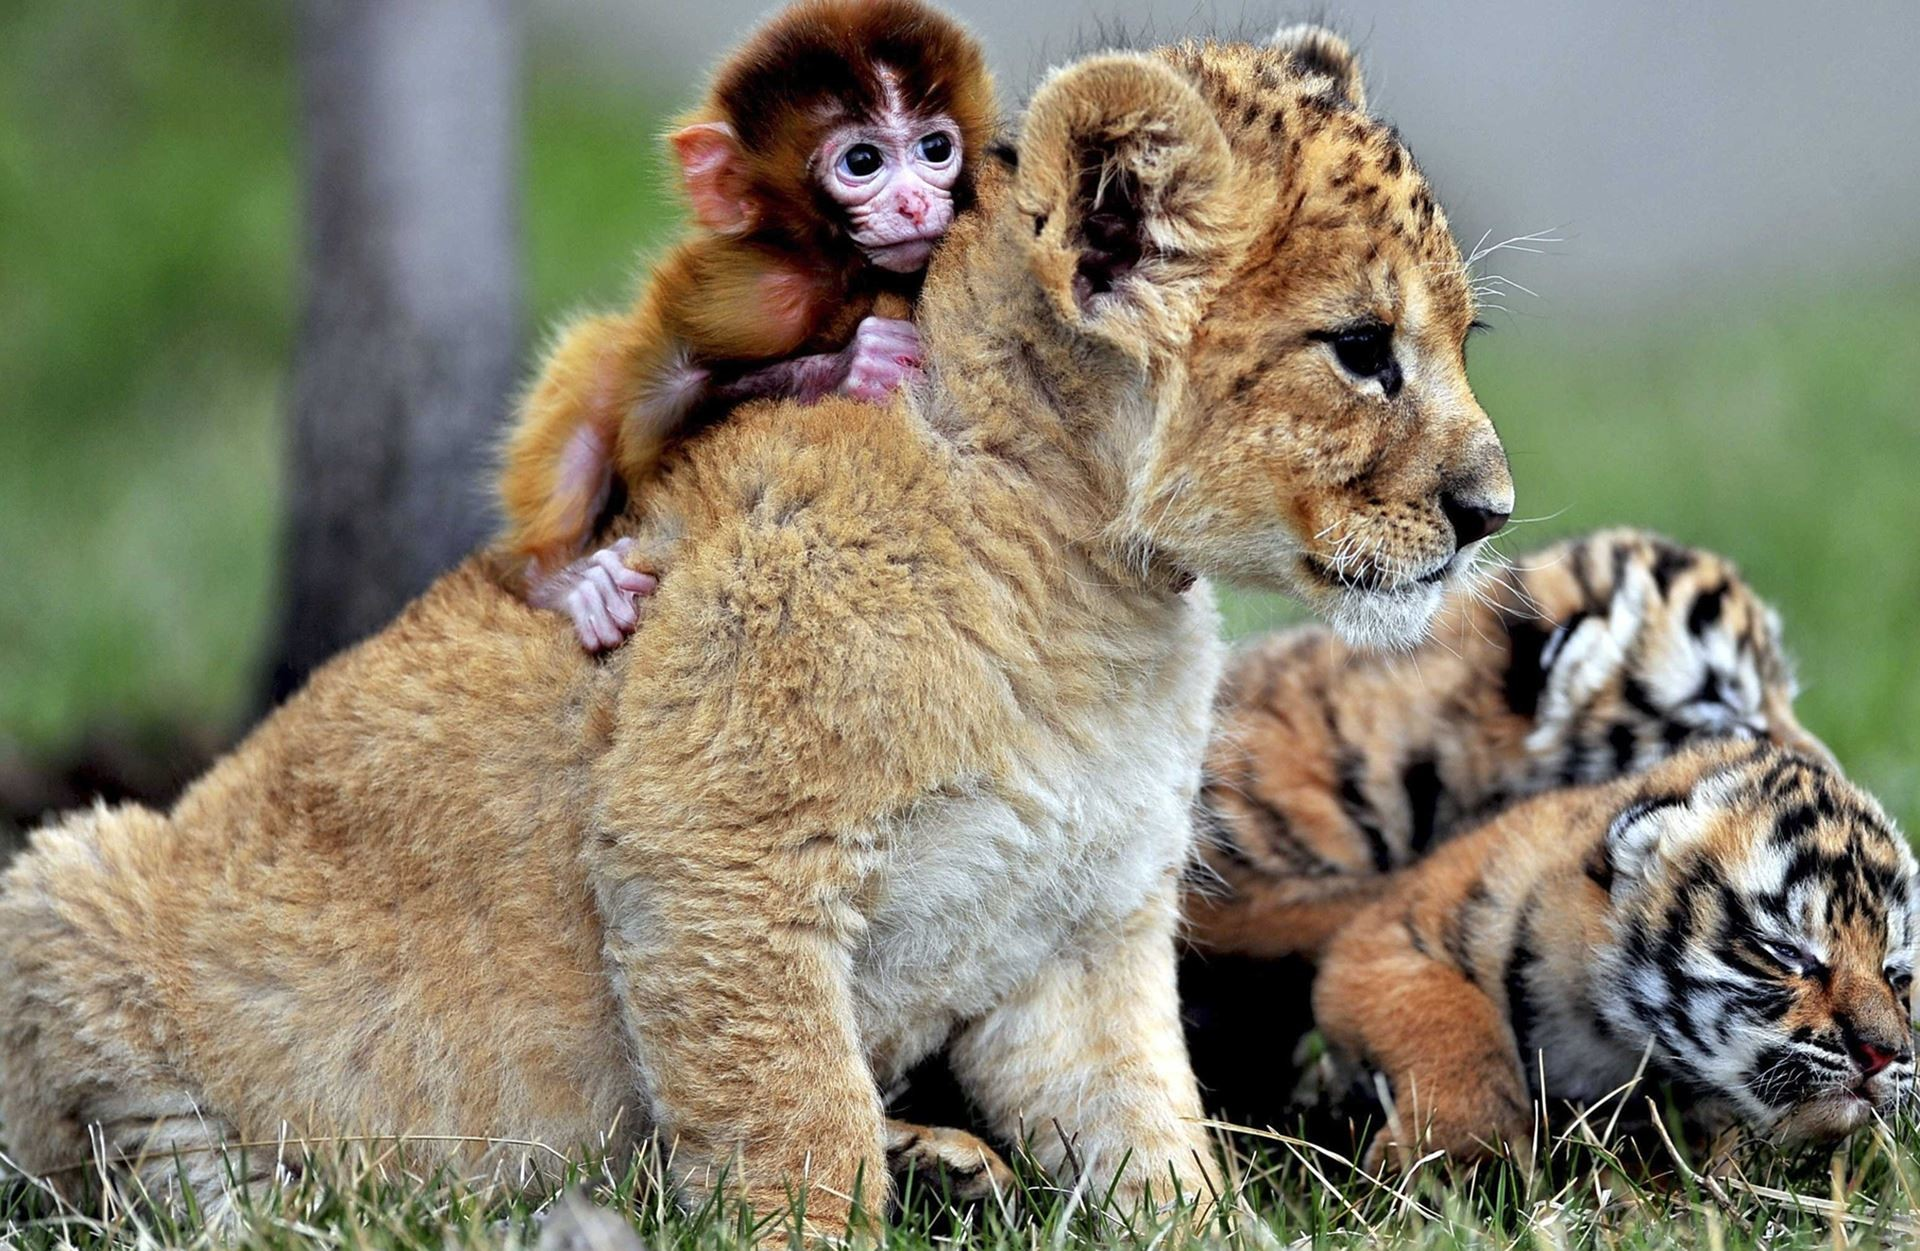
\includegraphics[width = 3.2in]{figures/TheConquistadorMonkey.eps}
	\caption{The Brave Monkey }
	\label{figConquistador}                         
\end{figure}  
	\chapter{Design} \label{chapter:design}

Here is the design.

\section{Feature Extraction}

\section{Thesis Modeling}

\section{Thesis Generation}

Other style for algorithms, it needs package algorithm. Currently it is in conflict with the package algorithm2e
\begin{comment}

\begin{figure}[h!]
\begin{algorithm}[H]
\caption{Get Maximum of Two Numbers}
\begin{algorithmic}[1]
\Procedure{GetMaximum}{$a, b$}
\If{$a \geq b$}
  \State \textbf{return} $a$
\Else
  \State \textbf{return} $b$
\EndIf
\EndProcedure
\end{algorithmic}
\end{algorithm}
\caption{Pseudo Code of GetMaximum}
\label{figure:pseudo_code_of_get_maximum}
\end{figure}
	content...
\end{comment}

The following is a equation example. There are many ways you can do it.
\begin{equation}\label{eq1}          
\begin{aligned}                        
	\underbrace{P(y_i = x|E)}_\text{yourtext} = \frac{1}{P(E)} \underbrace{P(E|y_i = x)}_\text{extr}\underbrace{P(y_i = x)}_\text{intr},
\end{aligned}                          
\end{equation}
Equation without number
\begin{equation*}\label{eq1p}          
%\begin{aligned}                        
	P_E^{p}(y_i = x) = P(y_i = x|E).     
%\end{aligned}                          
\end{equation*}
\begin{equation}\label{eq2}          
	\begin{aligned}                        
		z^{n} = \frac{x}{y}.     
	\end{aligned}                          
\end{equation}


	%\chapter{Implementation} \label{chapter:implementation}

\begin{figure}[h!]
\centering

\includegraphics[width=4cm,keepaspectratio]{figures/tensorflow.png}
\caption{TensorFlow's Logo}
\label{figure:tensorflow_logo}
\end{figure}

We implement the prototype on TensorFlow\cite{tensorflow} platform. Figure \ref{figure:tensorflow_logo} shows the logo of TensorFlow, and Figure \ref{figure:code_snippet_of_model_training} shows the code snippet of model training.

\begin{figure}[h!]
\begin{lstlisting}[language=python]
import tensorflow as tf

def train(total_loss, global_step):
  # Variables that affect learning rate.
  num_batches_per_epoch = NUM_EXAMPLES_PER_EPOCH / FLAGS.batch_size
  decay_steps = int(num_batches_per_epoch * NUM_EPOCHS_PER_DECAY)

  # Decay the learning rate exponentially.
  lr = tf.train.exponential_decay(INITIAL_LEARNING_RATE,
                                  global_step,
                                  decay_steps,
                                  LEARNING_RATE_DECAY_FACTOR,
                                  staircase=True)
  tf.summary.scalar('learning_rate', lr)
\end{lstlisting}
\caption{Code Snippet of Model Training}
\label{figure:code_snippet_of_model_training}
\end{figure}
	\chapter{Evaluation} \label{chapter:evaluation}

Here is the evaluation.

\section{Datasets}

\section{Experiment Design}

\section{Experimental Results}

\subsection{Training Time}

Table \ref{table:training_time} lists the training time of different datasets.

\begin{table}[h!]
\centering
\caption{Training Time}
\begin{tabular}{ |c|c| } 
\hline
\textbf{Dataset} & \textbf{Training Time} \\
\hline
\hline
A & 1 hour \\
\hline
B & 2 hours \\
\hline
C & 3 hours \\
\hline
D & 4 hours \\
\hline
E & 5 hours \\
\hline
\end{tabular}
\label{table:training_time}
\end{table}

\subsection{Example of Generated Thesis}

	\chapter{How to use citations} \label{labelIfyouWant}



\subsection{Biblatex}

From your favorite citation manager export a BibTeX library with the citations you need to \texttt{references/refs.bib}



\subsection{Compilation}

\begin{itemize}

   \item Compile document with XeLaTeX to write citations to \texttt{.aux} file\\ (i.e.\ xelatex ThesisTemplate.tex)

   \item Run biber on your document put the relevant entries into \texttt{.bbl} file\\ (i.e.\ biber ThesisTemplate)

   \item Compile document with XeLaTeX to include the \texttt{.bbl} file\\ (i.e.\ xelatex ThesisTemplate.tex)

   \item Compile document with XeLaTeX again to correctly label and include the citations\\ (i.e.\ xelatex ThesisTemplate.tex)

\end{itemize}



\subsection{Example}

Here are the related works~\cite{Chu2019}.


		\chapter{One way to write algorithms}
	
	\begin{algorithm}
		\DontPrintSemicolon
		\KwInput{Codeword from channel with the i$th$ element equal to $L(P_{V_i}^{int})$}
		\KwOutput{Decoded message $\hat{V}$ with the i$th$ element equal to $\hat{V_i}$}
		%\KwData{Testing set $x$}
		\tcp{Just comment this comment and the above Input and Output if not needed them}
		\textbf{Initialization:}\\
		\For {each $V_i$ in $\mathcal{V}$ }{
			$V_i$ = $L(P_{v_i}^{int})$
		}
		\textbf{Decoding:}\\
		\For {t = 1,..,Max Iterations}{
			\For {m = 1,..,Sub Iterations}{
				\textbf{Check Node Processing:}\\
				do something based on Eqn. (\ref{eq1})\\
				\textbf{Variable Node Processing:}\\
				Calculate $\gamma$ based on Eqn. (\ref{eq2})\\
				Check fo rearly termination or continue util max iter
			}
		}	
		\caption{Name of the Algorithm}
	\end{algorithm}
	\chapter{Conclusion} \label{chapter:conclusion}

You have compled your thesis, do whatever you please with your life.
	

	\begin{appendices}
		\chapter{First Appendix}
The is an appendix chapter. You can define more appendices in the same way.
\section{First Section}
The is an appendix session. You can define more sessions in the same way. 
	\end{appendices}
	
	\TSzTwelveTwenty\selectfont
\begin{thebibliography}{1}
	\bibliographystyle{plainnat}
	%\bibliographystyle{ieeetr}
	%\bibliography{bibfile}
	\bibitem{Gallager:1962}  %1
	R. G. Gallager, ``Low-density parity check codes," \emph{IRE Trans. on Information Theory,} vol. IT-8, pp.21-28, Jan. 1962. 
	\bibitem{Mackay:1999}   %2
	D. J. C. Mackay, ``Good error correcting codes based on very sparse matrices," IEEE Trans. on Inform. Theory, vol. 45, pp.399-43I, Mar.1999. 
	\bibitem{IEEE 802.11an}
	\emph{IEEE Standard for Information Technology – Telecommunications and
	Information Exchange between Systems – Local and Metropolitan Area
	Networks – Specific Requirements Part 3: Carrier Sense Multiple Access
	with Collision Detection (CSMA/CD) Access Method and Physical
	Layer Specifications,} IEEE Std. 802.3an, Sep. 2006.
	\bibitem{IEEE802.15.3c} %3
	\emph{Part 15.3:WirelessMedium Access Control (MAC) and Physical Layer (PHY) Specifications for High Rate Wireless Personal Area Networks(WPANs),} IEEE Std. P802.15.3c, 2009.
	\bibitem{IEEE802.11ad}  %4
	\emph{PHY/MAC Complete Proposal Specification, Std. IEEE 802.11-10/0433r,} IEEE 802.11 Task Group AD, May 2010.
	\bibitem{IEEE802.11ay}
	\emph{P802.11ay™/D3.0 Draft Standard for Information Technology –Telecommunications and Information Exchange Between Systems – Local and Metropolitan Area
	Networks – Specific Requirements – Part 11: Wireless LAN Medium Access Control (MAC) and Physical Layer (PHY) Specifications – Amendment 2: Enhanced throughput for operation in license-exempt bands above 45 GHz,} February, 2019.
	\bibitem{A. J. Blanksby} %5
	A. J. Blanksby and C. J. Howland, ``A 690-mW1-Gb/s 1024-b, rate-1/2 low-density parity-check code decoder," \emph{IEEE J. Solid-State Circuits,}
	vol. 37, no. 3, pp. 404–412, Mar. 2002.
	 \bibitem{M.P.C.Fossorier} %7
	M. P. C. Fossorier, M. Mihaljevic and H. Imai, ``Reduced complexity iterative decoding of low-density parity check codes based on belief propagation," \emph{in IEEE Transactions on Communications,} vol. 47, no. 5, pp. 673-680, May 1999.
	\bibitem{M.Whatever} %7
	whoever and whatever you put here
	\end{thebibliography}
	
	
\end{document}
